\documentclass[../../dissertation.tex]{subfiles}
\begin{document}

As was seen in section \ref{sec:chap3StagWalk}, the elements of each
tesselation of a discretely numbered cycle can be described by states
\begin{equation}
        \ket{\alpha_x} = \frac{\ket{2x} + \ket{2x+1}}{\sqrt{2}}
\end{equation}
\begin{equation}
        \ket{\beta_x} = \frac{\ket{2x+1}+\ket{2x+2}}{\sqrt{2}}.
\end{equation}
These states allow the construction of the Hamiltonians
\begin{equation}
        H_\alpha = 2\sum_{x=-\infty}^{+\infty}\ket{\alpha_{x}}\bra{\alpha_x} - I
\end{equation}
\begin{equation}
        H_\beta = 2\sum_{x=-\infty}^{+\infty}\ket{\beta_{x}}\bra{\beta_x} - I
\end{equation}
as was seen in equations \ref{eq:stagSimulHalpha} and \ref{eq:stagSimulHbeta}.
As was shown by \cite{acasiete2020}, these operators cane be rewritten in
matrix form 
\begin{equation}
	H_\alpha = I \otimes X
\end{equation}
%TODO: ESCREVER EQUACAO MATRICIAL DO HBETA
\begin{equation} 
	H_\beta = 
\end{equation} 
which are very useful representations when constructing the circuit.\par 

As was shown in equation \ref{q:stagSimulUniOp}, the unitary evolution operator
is
%TODO: DESCOBRIR SE A OS US ESTAO NA ORDEM CORRETA. 
\begin{equation}
	U = e^{i\theta H_\beta}e^{i\theta H_\alpha} = U_\beta U_\alpha, 
\end{equation} 
and knowing that
%TODO: TENTAR DESCOBRIR MELHOR MANEIRA DE REPRESENTAR ISTO. SERA QUE PRECISO DA MATRIZ TODA?  
\begin{equation} 
	R_x(\theta) = e^{\frac{-i\theta X}{2}}, 
\end{equation} 
then each of the operators associated with the different tesselation
Hamiltonians can be written as
\begin{equation} 
	U_\alpha = I \otimes R_x(\theta) 
\end{equation}
%TODO: Escrever Beta
\begin{equation} 
	U_\beta = 
\end{equation}
Notice that $U_\beta$ is simply a permutation of $U_\alpha$ and can be rewritten as
\begin{equation}
	U_\beta = P^{-1} U_\alpha P
\end{equation}
where $P = \sum_x \ket{x+1}\bra{x}$. Remember from equation
\ref{eq:shiftMatrixQiskit} and figure \ref{fig:coinedIncrement} that these
permutation operators can be implemented as increment and decrement gates, as
was proposed by \cite{douglaswang07}. Therefore, the circuit for the
staggered quantum walk on the line can be constructed as is shown in figure
\ref{fig:stagQWCirc}. 
\begin{figure}[!h]
	\[ \Qcircuit @C=1em @R=0.7em {   & & && \mbox{Repeat for the number of steps} & &\\ \\
	               &       & \qw & {/^{\otimes n-1}}\qw      & \multigate{1}{INCR}&\qw &  \multigate{1}{DECR} & \qw \\
            	   &       &\qw & \gate{R_x(2\theta)}    & \ghost{INCR} &\gate{R_x(2\theta)}        & \ghost{DECR} & \qw \gategroup{3}{4}{4}{7}{.8em}{--}
		          } \]
	\caption{stagqw}
	\label{fig:stagQWCirc}
\end{figure}\par

The next step is to implement the circuit in Qiskit, in order to test it in a real quantum computer. Here, the walk will take place in a cyclic graph with $8$ elements, meaning 3 qubits will be required as is shown in figure \ref{fig:stagQWCircuitQistkit}.
\begin{figure}[!h]
	\centering
	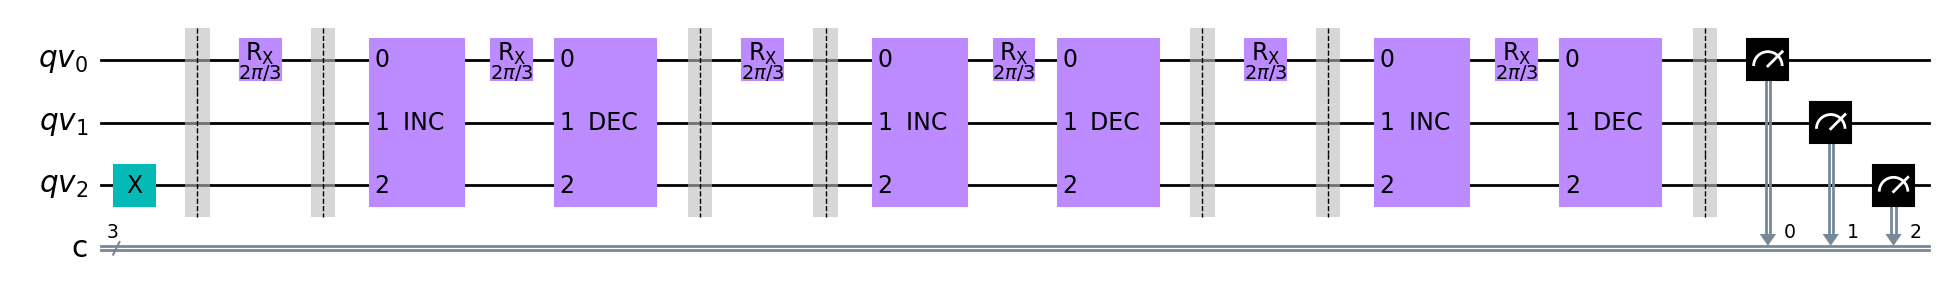
\includegraphics[scale=0.32]{img/Qiskit/StaggeredQW/Circuits/circStagQW_N3_S3.png}
	\caption{Temp} 
	\label{fig:stagQWCircuitQistkit}
\end{figure}\par
The circuit starts with a Pauli-X gate in the third qubit so that $\ket{\psi_0}
= \ket{4}$. The following operation is a rotation in the X basis, where $\theta
= \frac{\pi}{3}$ since it was seen in figure \ref{fig:stagQWSimulMultTheta}
that this value of $\theta$ maximizes the propagation of the walk. Finally,
$U_\beta$ is applied, making use of the increment and decrement gates defined
in figures \ref{fig:incrCircuitQistkit} and \ref{fig:decrCircuitQistkit}. This
procedure is repeated $3$ times, and the resulting probability distributions
after measurement can be seen in figure \ref{fig:stagQWQiskitDist}. 
\begin{figure}[!h]
	\centering
	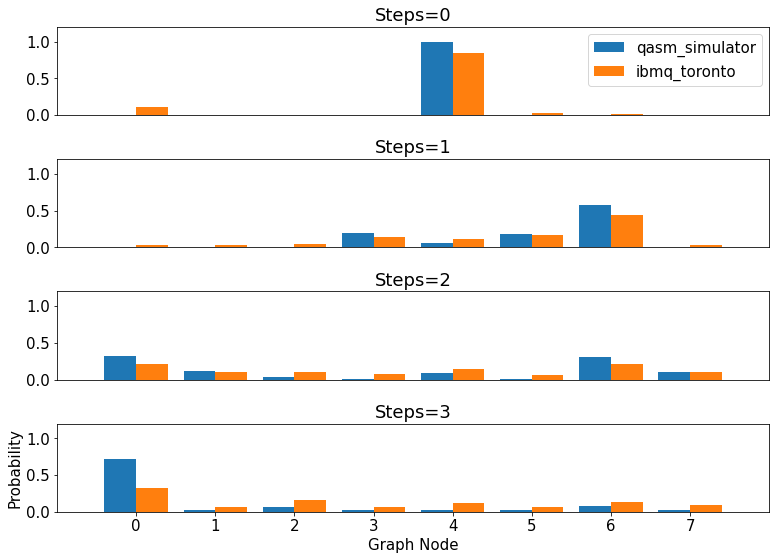
\includegraphics[scale=0.40]{img/Qiskit/StaggeredQW/StagQW_N3_S0123.png}
	\caption{Temp} 
	\label{fig:stagQWQiskitDist}
\end{figure}

\end{document}
